% !TEX root = ./Vorlesungsmitschrift DIFF 2.tex  
\lecture{Mo 17.05. 10:15}{}
\begin{beispiele*}[Weitere zum Satz über implizite Funktionen]
  \begin{enumerate}
    \item \( f\maps \reals^3\to \reals^2 \), \( f(x,y,z)=\begin{pNiceMatrix} x^2-y^2+1 \\ x^2-z^2-2 \end{pNiceMatrix} \) ist stetig differenzierbar.
    \begin{equation*}
      \totalderivative-{f}(x,y,z)=\begin{pNiceMatrix} 2x & -2y & 0 \\ 2x & 0 & -2z \end{pNiceMatrix}.
    \end{equation*}
    Ist  \( y_0\cdot z_0\neq 0 \) (also beide \( \neq 0 \)), so ist \( -2 \begin{pNiceMatrix} y_0 & 0 \\ 0 & z_0 \end{pNiceMatrix} \) invertierbar.

    Es gibt also ein offenes Intervall \( I \), \( x_0\in I \) und eine offene Umgebung \( V_2 \) von \( \begin{pNiceMatrix} y_0 \\ z_0 \end{pNiceMatrix}\in \reals^2\setminus \text{Achsen} \) und eine stetig differenzierbare Funktion \( g\maps I\to \reals \) mit \( g(I)\subset V_2 \) \sd
      \begin{equation*}
        f(x,y,z)=C=f(x_0,y_0,z_0)\iff  \begin{pNiceMatrix} y \\ z \end{pNiceMatrix}=g(x)
      \end{equation*}
      und es gilt 
      \begin{equation*}
      g'(x)=\frac{1}{2}\begin{pNiceMatrix} \frac{1}{y} &  \\  & \frac{1}{z} \end{pNiceMatrix}\begin{pNiceMatrix} 2x \\ 2x \end{pNiceMatrix}=\begin{pNiceMatrix} x/g_1(x) &  \\  & x/g_2(x) \end{pNiceMatrix},
      \end{equation*}
      also \( g_1'(x)g_1(x)=x\) und \( g_2'(x)g_2(x)=x \). Hauptsatz der Differential- und Integralrechnung 
      \begin{align*}
        \implies &\equalto{\text{(Substitution)}\ \Integrate{u}{u,g_j(x_0),g_j(x)}=\frac{1}{2}(g_j^2(x)-g_j^2(x_0))}{\Integrate{g_j'(t)g_j(t)}{t,x_0,x}}=\frac{x^2}{2}-\frac{x_0^2}{2}\quad j=1,2\\
        \implies \begin{aligned}[t]
          x^2>x_0^2-y_0^2&\maps g_1(x)=\sgn{y_0}\sqrt{x^2-x_0^2+y_0^2}\\
          x^2>x_0^2-y_0^2&\maps g_2(x)=\sgn{z_0}\sqrt{x^2-x_0^2+z_0^2}.
        \end{aligned}
      \end{align*}
      \begin{beispiel*}
        Für \( (x_0,y_0,z_0)=(3,2,-1) \)
        \begin{equation*}
          g\maps \ointerval{2\sqrt{2}}{\infty}\to \reals^2\quad g(x)=\begin{pNiceMatrix} \sqrt{x^2-5} \\ -\sqrt{x^2-8} \end{pNiceMatrix}
        \end{equation*}
        \begin{figure}[H]
          \centering
          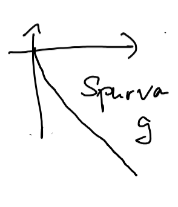
\includegraphics[width=0.2\linewidth]{figures/implizite_funktion_1_zu_2d_beispiel_spur}
          \label{fig:implizite_funktion_1_zu_2d_beispiel_spur}
        \end{figure}
      \end{beispiel*}
      \item \( f\maps \reals^n\times \reals\to \reals \), \( f(x,t)=t^n+\sum_{j=1}^{n}x_j t^{n-j} \), \( f(x,t)=0 \) \timplies \( t \) Nullstelle des Polynoms \( p_x(t)=f(x,t) \).

      Sei \( t_0 \) eine einfache Nullstelle. Dann ist \( D_2f(x,t_0)\neq 0 \), da \( p_x(t)=(t-t_0)q_x(t) \) und \( q_x(t_0)\neq 0 \) und somit \( D_2f(x,t_0)=q_x(t_0)+\cancel{(t_0-t_0)q_x'(t_0)} \).

      \timplies \texists  Umgebung \( U \) von \( x_0\in \reals^n \) und ein stetig differenzierbare Funktion \( g\maps U\to \reals \) mit \( f(x,g(x))=0 \) und \( g(x_0)=t_0 \) \timplies Die einfachen Nullstellen eines Polynoms hängen in stetig differenzierbarer Art von den Koeffizienten ab, \dh insbesondere hängen si stetig davon ab, \dh zu \( \varepsilon>0 \), \texists \( \delta>0 \) \sd \( \abs{t-t_0}=\abs{g(x)-g(x_0)}<\varepsilon \) für \( x\in B_\phi(x_0)\subset U \). 
      \begin{beispiel*}
        \begin{description}
          \item[\( 3t^2-t \)] Einfache Nullstelle \( t_0=\frac{1}{3} \).
          \item[\( \frac{10}{3}t^2-t \)] Einfache Nullstelle \( t_0=\frac{3}{10} \). 
        \end{description}
      \end{beispiel*}
      \item Die Bedingung im Satz über implizite Funktionen ist \emph{nicht} notwendig. \( f(x,y)=y^2 \) erfüllt in \( (1,0) \) die Bedingung \( D_2 f(1,0) \) invertierbar \emph{nicht}, \( f(x,y)=0 \) besitzt aber die Auflösung \( g(x)=0\quad \forall 0 \).
  \end{enumerate}
\end{beispiele*}
\section*{Der Satz von der Umkehrabbildung}\label{satz_von_der_umkehrabbildung}
Sei \( f\maps U\to \reals^n \) stetig differenzierbar, \( U\subset \reals^n \). Gibt es einfach zu prüfende Kriterien, die garantieren, dass \( f \) umkehrbar ist mit stetig differenzierbarer Umkehrfunktion \( g\maps f(U)\to \reals^n \)?

Notwendiges Kriterium ist, dass \( \totalderivative-{f}(x) \) invertierbar ist, da mit der Kettenregel aus \( g\circ f=\Id_u \) folgt \( \totalderivative-{g}(f(x))\matrixmult \totalderivative-{f}(x)=\mathds{1} \). Tatsächlich ist sogar folgendr hinreichend:

\begin{satz}
  Sei \( U\subset \reals^n \) offen, \( f\maps U\to \reals^n \), stetig differenzierbar. Sei \( a\in U \) \sd \( \totalderivative-{f}(a) \) invertierbar ist. Dann gibt es eine offene Umgebung \( V\subset U \) von \( a \) und eine offene Umgebung \( W\in \reals^n \) von \( b\definedas f(a) \), \sd \( f\maps V\to \reals^n \), \( V \) bijektiv auf \( W \) abgebildet und die Umkehrabbildung \( g\maps W\to \reals^n \) stetig differenzierbar ist. Es gilt dann
  \begin{equation*}
    \totalderivative-{g}(f(x))=\inverse{\totalderivative-{f}(x)}\quad \forall x\in V.
  \end{equation*}
\end{satz}
\begin{bemerkung*}
  Die letzte Identität, die wir obn schon bewiesen hatten, leuchtet unmittelbar ein, wenn man sich überlegt, dass die Ableitung eine differenzierbare Funktion linear approximiert, und dass die Umkehrabbildung einer invertierbaren linearen Abbildung die inverse Matrix ist.
\end{bemerkung*}
\begin{proof}[Beweis von \ref{satz_von_der_umkehrabbildung}]
  Betrachte \( F\maps \reals^n\times U\to \reals^n \), \( \distance{z}{x}=z-f(x) \). Dann ist 
  \begin{equation*}
    \totalderivative{f}(z,x)=(\underbrace{\mathds{1}_{n\times n}}_{D_1 F(z,x)}-\underbrace{\totalderivative{f}(x)}_{D_2 F(z,x)}).
  \end{equation*} 
  Wegen \( F(b,a)=0 \) und \( D_2 F(b,a)=-\totalderivative-{f}(a) \) invertierbar können wir den Satz von der impliziten Funktion \ref{satz_von_der_impliziten_funktion} auf \( F \) anwenden und \( F \) nach \( x \) auflösen. Es gibt also offene Umgebungen \( V_1\subset \reals^n \) von \( b \) und \( V_2\subset U \) von \( a \) und eine stetig differenzierbare Funktion (\vgl Bemerkung~\ref{implizite_funktion_auf_umgebung_stetig_differenzierbar} nach    \ref{satz_von_der_impliziten_funktion}) \( g\maps V_1\to \reals^n \) mit \( g(V_1)\subset V_2 \) und \( F(z,g(z))=0\quad \forall z\in V_1 \), also \( z-f(g(z))=0 \quad \forall z\in V_1 \) und für all \( (z,x)\in V_1\times V_2 \) mit \( F(z,x)=0 \) gilt \( x=g(z) \).

  Setze nun
  \begin{gather*}
    V \begin{aligned}[t]
      &\definedas V_2\cap \explain{\text{Urbild von \( V_1 \)}}{\inverse{f}(V_1)}\\
      &=\Set{x\in V_2|f(x)\in V_1}.
    \end{aligned}
  \end{gather*}
  \( V \) ist offen (da \( f \) stetig und \( V_1,V_2 \) offen) und \( f \) bildet \( V \) bijektiv auf \( W\definedas V_1 \) ab und die Umkehrabbildung ist \( g \).
\end{proof}

Man sagt, wenn \( f \) wie oben ist: \enquote{\( f \) ist bei \( a \) \emph{lokal} umkehrbar.}
\begin{beispiele}
  \begin{enumerate}
    \item \( f(x)=\ln x \), \( x>0 \), \( a=1 \), \( b=0 \), \( f'(1)=1 \).
    \begin{figure}[H]
      \centering
      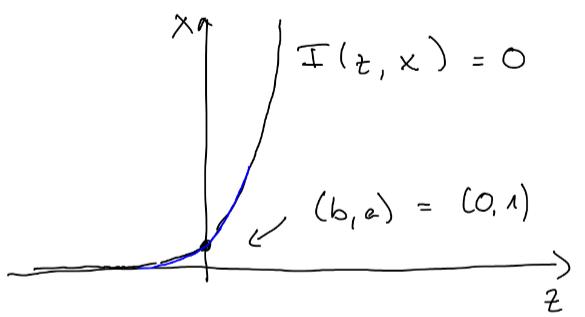
\includegraphics[width=0.5\linewidth]{figures/satz_von_der_umkehrungsfunktion_beispiel_ln}
      \caption*{\textcolor{Blue}{\( \Gamma_g=\Set{(z,g(z))|z\in V} \)}}
      \label{fig:satz_von_der_umkehrungsfunktion_beispiel_ln}
    \end{figure}
    \begin{gather*}
      g'(\ln x)=\inverse{\left( \frac{1}{x} \right)}=x\\
      g'(z)=g(z)\\
      \underset{(\text{\diff{1}})}{\implies} g(z)=C\exp (z),
    \end{gather*}
    und wegen \( g(0)=1 \) folgt \( C=1 \).
    \item \( f(x)=3x^2-x \), \( f(1)=2 \), \( \totalderivative-{f}(1)=5\neq 0 \).
    \begin{figure}[H]
      \centering
      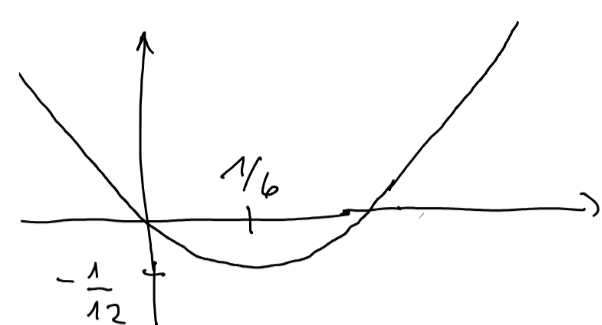
\includegraphics[width=0.5\linewidth]{figures/satz_von_der_umkehrungsfunktion_beispiel_parabel}
      \label{fig:satz_von_der_umkehrungsfunktion_beispiel_parabel}
    \end{figure}
    \begin{equation*}
      F(z,x)=z-f(x)\qquad N_f(0)=\Set{(f(x),x)|x\in U}
    \end{equation*}
    \begin{figure}[H]
      \centering
      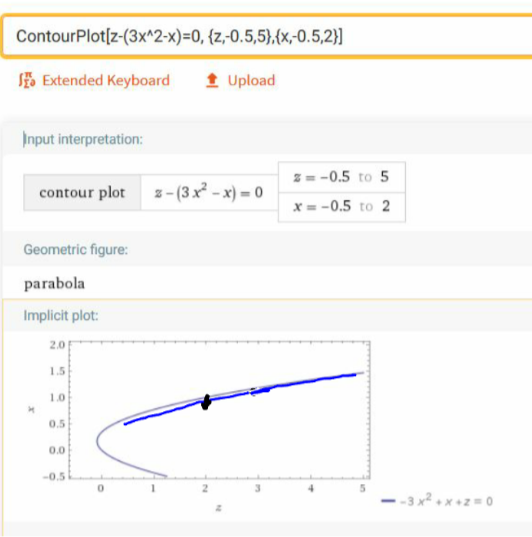
\includegraphics[width=0.5\linewidth]{figures/satz_von_der_umkehrungsfunktion_beispiel_parabel_umkehrung}
      \caption*{\( N_F(0) \), \textcolor{Blue}{\( \Gamma_g=\set{\underbrace{(z,g(z))}_{=(f(x),x)}|z\in W} \)}, von Wolfram Alpha.}
      \label{fig:satz_von_der_umkehrungsfunktion_beispiel_parabel_umkehrung}
    \end{figure}
    Die Rekursionsformel \( g_0(z)=a \), \( g_{j+1}(z)=a+h(z,g_j(z)) \),
    \begin{equation*}
      h(z,x)=x-\inverse{D_2 F(b,a)}\matrixmult F(z,x)
    \end{equation*}
    ist meist nicht sehr nützlich zur Bestimmung von \( g \). Aber die Ableitung von \( g \) können wir sofort bestimmen: \( \totalderivative-{g}(z)=\inverse{\totalderivative-{f}(g(z))} \) oder \( \totalderivative-{g}(f(x))=\inverse{\totalderivative-{f}(x)} \).

    Im Beispiel: \( g'(z)=\frac{1}{6g(z)-1} \) für \( g(z)\neq \quot{1}{6} \). \timplies Ansatz \( g(z)=\alpha+\sqrt{\beta+\gamma z} \)
    \begin{gather*}
      z\needed{=}f(g(z))=3(\alpha^2+\beta+\gamma z+2a\sqrt{\beta+\gamma z})-\alpha-\sqrt{\beta+\gamma z}\\
      \implies \begin{gathered}
        6\alpha = 1\\
        3\alpha^2+3\beta-\alpha=0\\
        3\gamma=1
    \end{gathered}\implies g(z)=\frac{1}{6}+\frac{1}{6}\sqrt{+1+12z}
    \end{gather*}
    auf \( \ointerval{-\frac{1}{12}}{\infty} \) definiert \timplies es muss \( f>-\frac{1}{12} \) sein, also ist das maximale \( V=\ointerval{\frac{1}{12}}{z} \).
    \item \( f\maps \reals_{>0}\times \reals\to \reals^2 \), \( (r,\phi)\mapsto \transpose{(r\cos \phi, r\sin \phi)} \).
    \begin{gather*}
      \Det \totalderivative-{f}(r,\phi)=\begin{pNiceMatrix} \cos \phi & -r\sin \phi \\ \sin \phi
       & r\cos \phi \end{pNiceMatrix}\\
       \Det \totalderivative-{f}(r,\phi)=r>0\quad \forall (r,\phi).
    \end{gather*}
    \timplies Bei allen \( r,\phi \) ist \( f \) lokal invertierbar. Es gilt
    \begin{equation*}
      \inverse{\totalderivative-{f}(r,\phi)}=\begin{pNiceMatrix} \cos \phi & \sin \phi \\ -\frac{\sin \phi}{r} & \frac{\cos \phi}{r} \end{pNiceMatrix}.
    \end{equation*}
    Setze \( f(r,\phi)=\begin{pNiceMatrix} x \\ y \end{pNiceMatrix} \) \timplies \( r=\sqrt{x^2+y^2} \), \( \frac{x}{r}=\cos \phi \), \( \frac{y}{r}=\sin \phi \).
    \begin{equation*}
      \implies \inverse{\totalderivative-{f}(r,\phi)}=\totalderivative-{f}(\underbrace{f(r,\phi)}_{=\begin{pNiceMatrix} x \\ y \end{pNiceMatrix}})=\begin{pNiceMatrix} \frac{x}{\sqrt{x^2+y^2}} & \frac{y}{\sqrt{x^2+y^2}} \\ \frac{-y}{x^2+y^2} & \frac{x}{x^2+y^2} \end{pNiceMatrix}
    \end{equation*}
    mit \( g  \) eine lokale Umkehrung.

    \begin{beachte*}
      \( f(\reals_{>0}\times \reals)=\reals^2\setminus \zeroset \), aber es gibt \emph{keine } globale Umkehrfunktion \( g\maps \reals^2\setminus \zeroset \to \reals^2 \), denn \( f(r,\phi+k2\pi)=f(r,\phi) \quad \forall k\in \wholes \), also \( f \) nicht injektiv. Man kann maximal Intervalle der Länge \( 2\pi \) (in \( \phi \)) betrachten.

      Betrachte etwa \( U=\reals_{>0}\times \ointerval{-\pi}{\pi} \). Das wird unter \( f \) bijektiv auf \( W=\reals^2\setminus \Set{(x,0)|x\leq 0} \) abgebildet.
      \begin{figure}[H]
        \centering
        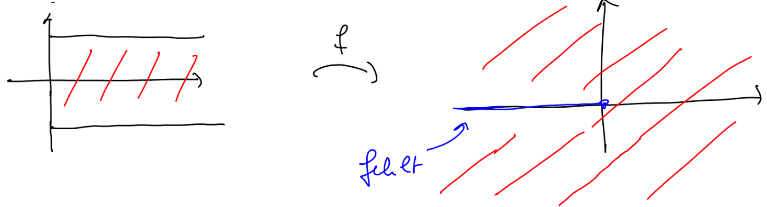
\includegraphics[width=0.5\linewidth]{figures/geschlitzte_ebene}
        \caption*{\enquote{geschlitzte Ebene}}
        \label{fig:geschlitzte_ebene}
      \end{figure}
      Wie kommt man darauf, dass \( f \) \( V \) auf \( W \) abbildet? \( \phi \) ist entweder \( \neq 0 \), dann ist \( r\sin \phi\in \ointerval{-r}{0}\cup \ointerval{0}{r} \), oder \( \phi=0 \), dann ist \( r\cos \phi=r>0 \).

      \minisec{\( \evaluateat{f}{U} \) ist injektiv:} Ist \( r\cos \phi=r'\cos \phi' \) und \( r\sin \phi=r'\sin \phi' \), so ist \( r^2=r'^2 \) \timplies (da, \( r,r'>0 \)) \( r=r' \) und aus \( \cos \phi=\cos \phi' \) folgt zunächst \( \phi=\pm \phi' \), aber aus \( \sin \phi=\sin \phi'=\pm \sin \phi \)folgt \( \phi=+\phi' \).

      \minisec{\( \evaluateat{f}{U} \) bildet surjektiv auf \( W \) ab:} Sei \( \begin{pNiceMatrix} x \\ y \end{pNiceMatrix} \in W \), \dh es ist \( y\neq 0 \) oder \( x>0 \) \timplies \( r=\set{x^2+y^2}>0 \) \timplies \( \left( \frac{x}{r} \right)^2+\left( \frac{y}{r} \right)^2=1 \) \timplies \( \abs{\quot{x}{r}}\leq 1 \). Es ist \( \quot{x}{r}\neq -1 \), denn sonst wäre \( \quot{y}{r}=0 \), aber \( (-1,0)\notin W \). Somit ist \( y=0 \) \tiff \( \quot{x}{r}=1 \) und wir legen einen Winkel \( \phi \) fest mit \( \cos \phi=\quot{x}{r} \). \( \phi\in \ointerval{-\pi
        }{0} \), falls \( y<0 \), oder \( \ointerval{0}{\pi} \), alls \( y>0 \), oder \( \phi=0 \), falls \( y=0. \)

      \begin{behauptung*}
        Für diesen Winkel gilt \( \sin \phi=\quot{y}{r} \).
      \end{behauptung*}
      \begin{proof}
        \begin{equation*}
          \sin \phi=\sgn{\sin \phi}\sqrt{\sin^2 \phi}=\sgn{y}\sqrt{1-\cos^2 \phi}=\sgn{y}\sqrt{1-\quot{x^2}{r^2}}=\sgn{y}\quot{\abs{y}}{r}=\quot{y}{r}.
        \end{equation*}
      \end{proof}
      Ist man nicht an einer maximalen Umgebung von \( \ointerval{r_0}{\phi_0}  \) interessiert, kann man so schneller zum Ziel:

      Ist beispielsweise \( -\quot{\pi}{2}<\phi_0<\quot{\pi}{2} \) betrachte \( \phi\in \ointerval{-\quot{\pi}{2}}{\quot{\pi}{2}} \),woraus \( x>0 \) folgt, so dass man recht schnell rät, dass \( f \) \( V\definedas \reals_{>0}\times  \ointerval{-\quot{\pi}{2}}{\quot{\pi}{2}} \) bijektiv auf \( W=\reals_{>0}\times \reals \) abbildet, indem man sich überlegt, dass die Umkehrfunktion \( g \) durch \( g(x,y)=\transpose{(\sqrt{x^2+y^2}, \arctan \quot{y}{x})} \) gegeben ist (wohldefiniert für \( x>0 \)), da 
      \begin{equation*}
        g(r \cos \phi, r\sin \phi)=(r,\underbrace{\arctan \quot{\sin \phi}{\cos \phi}_{=\phi}})
      \end{equation*}
      und es ist klar, dass \( g \) \( W \) bijektiv au \( V \) abbildet, da \( \arctan\maps \reals\to \ointerval{-\quot{\pi}{2}}{\quot{\pi}{2}} \) bijektiv ist, \sd  wenn \( \arctan \quot{x}{y}=\arctan \quot{\tilde{x}}{\tilde{y}} \) gilt \( y=\quot{\tilde{yx}}{x} \) und dann
      \begin{equation*}
        \sqrt{x^2+y^2}=\sqrt{x^2+\frac{\tilde{y}^2 x^2}{\tilde{x}^2}}=\frac{x}{\tilde{x}}\sqrt{\tilde{x}^2+\tilde{y}^2}
      \end{equation*}
      nut gleich \( \sqrt{\tilde{x}^2+\tilde{y}^2} \), wenn \( x=\tilde{x} \) (und somit \( y= \tilde{y}\)) und \( \reals_{>0}\times\reals\ni (x,y)\mapsto \sqrt{x^2+y^2} \) bildet surjektiv auf \( \reals_{>0} \) ab (da streng monoton wachsend).
    \end{beachte*}
  \end{enumerate}
\end{beispiele}
Es folgen einige etwas tiefsinnigere Folgen aus dem Umkehrsatz.
\begin{satz}\label{offene_abbildungen_satz}
  Sei \( f\maps U\to \reals^n \) stetig differenzierbar, \( U\subset \reals^n \) offen. Sei \( V\subset U \) offen. Ist \( \totalderivative-{f}(x) \) invertierbar für alle \( x\in V \), so ist \( \evaluateat{f}{V} \) eine \emph{offene Abbildung}, \dh offene Teilmengen \( \subset V \) auf offene Mengen abgebildet.
\end{satz}
\begin{antibeispiel*}
  \( f\maps \ointerval{0}{1}\to \reals \), \( f(x)=1\quad \forall x \). \( f'(x)=0 \) nicht invertierbar. \( \Set{1} \) nicht offen in \( \reals \).
\end{antibeispiel*}
\begin{proof}[Beweis von \ref{offene_abbildungen_satz}]
  Sei \( \tilde{V}\subset U \) offen, dann ist \( \tilde{V}  \) auch offen \( U \). Sei \( b\in f(\tilde{V}) \). Wähle ein \( a\in \tilde{V} \) \sd \( b=f(a) \). Wende den Satz von der lokalen Umkehrfunktion auf \( \evaluateat{f}{\tilde{V}} \) an \timplies \texists  offene Umgebungen \( V_1\subset \tilde{V} \) und \( W\subset \reals^n \) von \( a \) beziehungsweise \( b \) \sd \( \evaluateat{f}{V_1} \) umkehrbar ist mit \( g\maps W\to \reals^n \) und insbesondere \( f \) \( V_1 \) bijektiv auf \( W \) abbildet. Somit gilt \( W=f(V_1)\subset f(\tilde{V}) \) und ist Umgebung von \( b \) \timplies \( f(\tilde{V}) \) ist offen.
\end{proof}
\begin{satz}[Minimum- / Maximum-Prinzip]\label{extremumprinzip}
  Sei \( f\maps U\to \reals^n \), \( U\subset \reals^n \), stetig differenzierbar. Sei \( V\subset U \) offen und sei \( \totalderivative-{f}(x) \) invertierbar für alle \( x\in V \). Dann gilt für die Funktion
  \begin{equation*}
    V\ni x\mapsto \norm{f(x)}
  \end{equation*}
  \begin{enumerate}
    \item \label{extremumprinzip:kein_maximum} Sie besitzt kein Maximum.
    \item \label{extremumprinzip:kein_minimum_wenn_nicht_null} Ist \( f(x)\neq 0\quad \forall x\in V \) besitzt sie kein Minimum.
  \end{enumerate}
\end{satz}
\begin{beachte*}
  Man kann den Beweis dieses Satzes auf \ref{extremum_notwendige_bedingung} zurückführen, obwohl \( \norm{\cdot} \) nur auf \( \reals^n\setminus \zeroset  \) partiell differenzierbar ist. Wir wollen hier dennoch anders vorgehen:
\end{beachte*}
\begin{proof}
  \begin{proofdescription}
    \item[\ref{extremumprinzip:kein_maximum}] Angenommen \( a \) ist Maximalstelle von \( \norm{f} \). Dann ist \( f(a)\neq 0 \), da sonst \( \norm{f(x)}=0\quad \forall x\in V \) und somit \( \evaluateat{f}{V}=0 \) und \( \totalderivative-{f}(x)=0\quad \forall x\in V \). \ref{offene_abbildungen_satz} \timplies \texists  \( \varepsilon>0 \) \sd \( B_{\varepsilon}(f(a))\subset f(V) \). Setze \( b\definedas f(a)+\rho f(a) \) mit\( \rho=\quot{\varepsilon}{2\norm{f(a)}} \) 
    \begin{align*}
      \implies &\norm{b-f(a)}=\rho\norm{f(a)}=\quot{\varepsilon}{2}<\varepsilon\\
      \implies &b\in B_{\varepsilon}\implies \exists x_0\in V  \logicspace \text{\sd}\logicspace b=f(x_0)\\
      \implies &\norm{f(x_0)}=\norm{b}=(1+\rho)\norm{f(a)}>\norm{f(a)}.
    \end{align*}
    \item[\ref{extremumprinzip:kein_minimum_wenn_nicht_null}] Analog mit \( b=f(a)-\rho f(a) \).
  \end{proofdescription}
  
\end{proof}
